\documentclass[10pt]{article}
\usepackage[margin=0.90in]{geometry}
\usepackage{amsmath,amssymb,amsthm,mathtools}
\usepackage{microtype}
\usepackage{graphicx}
\usepackage[hidelinks]{hyperref}
\usepackage{fontawesome5}
\usepackage{enumitem}
\setlist{leftmargin=1.15em,itemsep=0.15em,topsep=0.25em}
\setlength{\parindent}{0pt}
\setlength{\parskip}{0.20em}
\setlength{\textfloatsep}{0.8em}

\newtheorem{proposition}{Proposition}
\newtheorem{lemma}{Lemma}
\newtheorem{definition}{Definition}

\begin{document}

\begin{center}
{\LARGE \bfseries The Response Spectrum of Recursive Self-Improvement\par}
\vspace{0.15em}
{\large Collapse, neutral churn, and takeoff in synthetic LLM populations\par}
\vspace{0.75em}
{\large Jonathan R. Landers\par}
\vspace{0.25em}
{July 2026\par}
\vspace{0.15em}
{\small\href{https://github.com/jonland82/finite-response-kernels}{\faGithub\ Project Repository}\par}
\end{center}

\vspace{0.35em}

\begin{abstract}
A language model repeatedly exposed to its own outputs need not simply improve or collapse. We model recursive prompting as a stochastic transition on finite populations, with conditional drift locating collapse, stasis, neutral churn, and improvement on one spectrum. A fixed-weight experiment compares raw replacement, anchoring, diversity verification, and diversity-guided prompting, producing near-neutral drift, delayed collapse, and two forms of rapid improvement. Terminal gain records the outcome, a signed takeoff kernel records its delivery, and total response reveals reversals. A scalar control $\rho$ traces the response spectrum; differentiation with respect to $\rho$ gives its local dynamical direction. This is not recursive training: recursion supplies a channel, while selection determines its direction.
\end{abstract}

\section{Recursion is not an outcome}

A common proposal for model self-improvement uses an outer loop: the model generates candidate outputs, a rule selects which survive, and the survivors define the next round. Full self-training would train a successor on them. Here the weights remain fixed so we can isolate the generate--select--repeat stage.

The loop has no predetermined direction. Raw copying may lose rare patterns; a fixed anchor set may preserve individual features while concentrating repeated combinations; diversity filtering may expand valid variety. The resulting population can collapse, churn near baseline, or improve.

The model-collapse literature establishes one end of this spectrum: recursive data can lose distributional tails and misrepresent the source \cite{shumailov2024,alemohammad2024}. Recursion can instead remain stable or useful when real data accumulate or filtering favors good samples \cite{kazdan2025}. Selection defines the direction.

Earlier work motivates two clocks: complete recursive rounds and checkpoints inside one training run \cite{landersTakeoff,landersModal}. We study the first. Diversity is not identified with general capability; it is a transparent finite-state coordinate on which collapse, persistence, and expansion can all be measured.

\section{An output-state coordinate}

At recursive round $r\in\{0,1,\ldots\}$, let $X_r$ be the population of $n_r\le m=24$ valid records. Each record has $d=4$ categorical fields, each with $k=4$ allowed values. For nonempty $X_r$, let $p_{rj}(a)$ be the fraction of records whose field $j\in\{1,\ldots,d\}$ has value $a\in\{1,\ldots,k\}$. Define normalized mean marginal entropy
\begin{equation}\label{eq:entropy}
\bar H_r=\frac{1}{d\log k}\sum_{j=1}^{d}
\left[-\sum_{a=1}^{k}p_{rj}(a)\log p_{rj}(a)\right].
\end{equation}
where $\log$ is the natural logarithm and $0\log0:=0$. This equals one for uniform field marginals. Let $\operatorname{supp}_{\rm emp}(X_r)$ be the set of distinct records present in $X_r$ and define
\begin{equation}\label{eq:distinct}
D_r=\frac{|\operatorname{supp}_{\mathrm{emp}}(X_r)|}{n_r},
\end{equation}
and the declared composite response
\begin{equation}\label{eq:quality}
Q_r=\frac{1}{2}(\bar H_r+D_r).
\end{equation}
$D_r$ is occupancy, not full joint entropy; $|\cdot|$ denotes set size. For an empty population set $\bar H_r=D_r=Q_r=0$. Thus $Q_r=Q(X_r)$, where $Q$ is the state score defined by Eq.~\eqref{eq:quality}; retaining both components prevents it from hiding the mechanism.

Let $[k]=\{1,\ldots,k\}$, let $\Omega=[k]^d$ be the record space, and let $\mathcal X_{\le m}$ be the finite set of populations of at most $m$ records on $\Omega$; thus $Q:\mathcal X_{\le m}\to[0,1]$. Recursive prompting defines
\begin{equation}\label{eq:transition}
X_{r+1}\sim P_\xi(X_r,\cdot),\qquad
P_\xi(x,y)=\Pr\!\left\{\mathcal S_\xi(\mathcal G(x))=y\right\},
\end{equation}
for states $x,y\in\mathcal X_{\le m}$. Here $\Pr$ denotes probability, $\sim$ means ``is drawn from,'' and $P_\xi(x,\cdot)$ is the successor distribution from $x$. The matrix $P_\xi$ is determined by LLM generation $\mathcal G(x)$, successor rule $\mathcal S_\xi$, and intervention label $\xi$. Model weights stay fixed.

\section{The collapse--improvement spectrum}

For a state $x\in\mathcal X_{\le m}$, define the conditional drift
\begin{equation}\label{eq:drift}
b_\xi(x)=\mathbb E_\xi[Q(X_{r+1})-Q(X_r)\mid X_r=x].
\end{equation}
The subscript on $\mathbb E_\xi$ means that expectation is taken under transition law $P_\xi$, over model sampling and randomized selection. Thus $b_\xi(x)$ is the expected one-round score change from state $x$.

\begin{lemma}[Drift accumulation]\label{lem:drift}
For any positive integer horizon $R$ and fixed initial state,
\begin{equation}\label{eq:drift-sum}
\mathbb E_\xi[Q(X_R)-Q(X_0)]
=\sum_{r=0}^{R-1}\mathbb E_\xi[b_\xi(X_r)].
\end{equation}
Thus nonpositive drift on all visited states gives expected collapse, zero drift gives score-neutral propagation, and nonnegative drift gives expected improvement.
\end{lemma}

\begin{proof}
Write the terminal difference as a telescoping sum, condition each increment on $X_r$, and apply the tower property of conditional expectation.
\end{proof}

Neutrality has two geometries. \emph{Stasis} means $Q(X_r)$ barely moves. \emph{Churn} means positive and negative increments cancel, so the endpoint is nearly unchanged despite a long path. The distinction will be measured below by total variation.

\begin{lemma}[A bounded response must saturate]\label{lem:ceiling}
Because $0\le Q\le1$, if $b_\xi\ge0$ on visited states, then
\begin{equation}\label{eq:ceiling}
0\le\sum_{r=0}^{R-1}\mathbb E_\xi[b_\xi(X_r)]\le1-Q(X_0).
\end{equation}
If instead $b_\xi\le0$, the magnitude of the sum is at most $Q(X_0)$. In particular, drift of one sign cannot remain bounded away from zero indefinitely.
\end{lemma}

\begin{proof}
Combine Lemma~\ref{lem:drift} with $-Q(X_0)\le Q(X_R)-Q(X_0)\le1-Q(X_0)$.
\end{proof}

Now orient a scalar control $\rho$ from collapse through neutrality to improvement, and let $P_\rho$ be a differentiable path of transition matrices. This path could vary selection strength or randomize between successor rules. Write
\begin{equation}\label{eq:rho-trajectory}
q_r(\rho)=\mathbb E_\rho Q(X_r)=\mu_0P_\rho^rQ,
\qquad \bar\Delta_r(\rho)=q_r(\rho)-q_{r-1}(\rho),
\end{equation}
where $\mathbb E_\rho$ is expectation under $P_\rho$, $q_r$ is expected score, $\bar\Delta_r$ is its expected increment, $\mu_0$ is the row vector of initial-state probabilities, $P_\rho^r$ is the $r$-step transition matrix, and $Q$ is the column vector of state scores. Define expected terminal gain $\bar g_R(\rho)=q_R(\rho)-q_0(\rho)$.

\begin{lemma}[Recursive susceptibility]\label{lem:susceptibility}
With $s$ indexing the affected stage, the derivative $\chi_r(\rho)=\partial_\rho q_r(\rho)$ satisfies
\begin{equation}\label{eq:duhamel}
\chi_r(\rho)=\sum_{s=0}^{r-1}
\mu_0P_\rho^s(\partial_\rho P_\rho)
P_\rho^{r-1-s}Q.
\end{equation}
Consequently the tangent response kernel
\begin{equation}\label{eq:tangent-kernel}
\tau_r(\rho)=\partial_\rho\bar\Delta_r(\rho)
=\chi_r(\rho)-\chi_{r-1}(\rho)
\end{equation}
obeys $\sum_{r=1}^{R}\tau_r=\partial_\rho\bar g_R$.
\end{lemma}

\begin{proof}
Differentiate $P_\rho^r$ by the product rule, inserting $\partial_\rho P_\rho$ at each possible recursive stage; the kernel identity then telescopes.
\end{proof}

Equation~\eqref{eq:duhamel} is the discrete linear-response formula: a change in $\rho$ can enter at stage $s$ and propagate through the remaining rounds. Write $\bar\Delta=(\bar\Delta_1,\ldots,\bar\Delta_R)$ and $\tau=(\tau_1,\ldots,\tau_R)$. Then $\rho\mapsto\bar\Delta(\rho)$ traces a curve in response-kernel space and $\tau(\rho)$ is its tangent. For $\ell$ controls $\boldsymbol\rho=(\rho_1,\ldots,\rho_\ell)$, the columns $\partial_{\rho_j}\bar\Delta$ span the locally accessible dynamical subspace. This unnormalized form remains regular at a neutral point $\bar g_R=0$, where division by $|\bar g_R|$ is singular.

\section{Path shape: a signed takeoff kernel}

For a positive integer horizon $R$ and rounds $r=1,\ldots,R$, define the realized increment and terminal gain
\begin{equation}\label{eq:increments}
\Delta_r=Q_r-Q_{r-1},\qquad g=Q_R-Q_0.
\end{equation}
When $g\ne0$, define $\operatorname{sign}(g)=g/|g|$ and the signed normalized takeoff kernel
\begin{equation}\label{eq:kernel}
\kappa_r=\frac{\Delta_r}{|g|},\qquad
\sum_{r=1}^{R}\kappa_r=\operatorname{sign}(g).
\end{equation}
The sign of $g$ places a realized run on the collapse--improvement spectrum; $g\approx0$ includes both stasis and churn. The kernel describes when that outcome arrives, and its signs may mix when a recursion regresses or recovers. No exponential law is assumed.

The finite-horizon geometry follows from a bookkeeping identity.

\begin{proposition}[Boundary and interior of recursive response]\label{prop:geometry}
For a real number $z$, let $(z)_+=\max\{z,0\}$. Define
\[
A_+=\sum_{r=1}^{R}(\Delta_r)_+,
\qquad A_-=\sum_{r=1}^{R}(-\Delta_r)_+,
\qquad A=\sum_{r=1}^{R}|\Delta_r|.
\]
These are positive, negative, and total path variation. They satisfy
\begin{equation}\label{eq:decomposition}
g=A_+-A_-,\qquad A=A_++A_-,\qquad
A_+=\frac{A+g}{2},\quad A_-=\frac{A-g}{2}.
\end{equation}
Consequently $A\ge |g|$, with equality if and only if all nonzero increments have the same sign.
\end{proposition}

\begin{proof}
Apply $z=(z)_+-(-z)_+$ and $|z|=(z)_++(-z)_+$ to every increment. Summing gives the first two identities; solving yields \eqref{eq:decomposition}. Triangle equality holds exactly when increments do not cancel.
\end{proof}

The lower wall $A=|g|$ contains monotone response. The interior $A>|g|$ contains overshoot, regression, or ringing. The excess
\begin{equation}\label{eq:excess}
E=A-|g|
\end{equation}
is response spent without surviving at the endpoint. This parallels the sharp boundary and broadened interior in \emph{The Entropy of Finite Response} \cite{landersEntropy}. There passive convolution imposes the geometry; here it describes signed paths. It is an analogy, not an LLM conservation law.

\section{The experiment inside the formalism}

The initial count profile was $(12,6,4,2)$ in every field, arranged so that $\bar H_0=0.8648$, $D_0=0.8750$, and $Q_0=0.8699$. Amazon Nova Lite generated ten rounds in 16 replicates. Each arm defines a different $P_\xi$; $b_{\rm raw}$ and $b_{\rm anchor}$ below denote Eq.~\eqref{eq:drift} for the named arms.

\begin{itemize}
\item \textbf{Raw replacement} uses an identity successor rule on 24 imitative generations. If imitation is score-preserving, $b_{\rm raw}\approx0$; sampling can still create churn.
\item \textbf{Fixed anchors} combines 18 generations with six fixed diverse records. Marginals should be protected, but $b_{\rm anchor}$ is ambiguous because a narrow archive may repeat correlations.
\item \textbf{Diversity verification} generates 36 candidates and greedily rewards underrepresented field values and unseen combinations while retaining 24. Since selection targets the ingredients of $Q$, positive early drift and ceiling saturation are expected.
\item \textbf{Diversity guidance} asks generation itself for even marginals and many combinations. It should bias drift positive, but less mechanically than post-generation selection.
\end{itemize}

The scaled run made 640 successful calls with no API errors. It used 344,406 input and 332,067 output tokens, with an estimated cost of $\$0.10036$ at the public rates encoded by the experiment. Error bands in Fig.~\ref{fig:curves} are standard errors over replicates.

\begin{figure}[t]
\centering
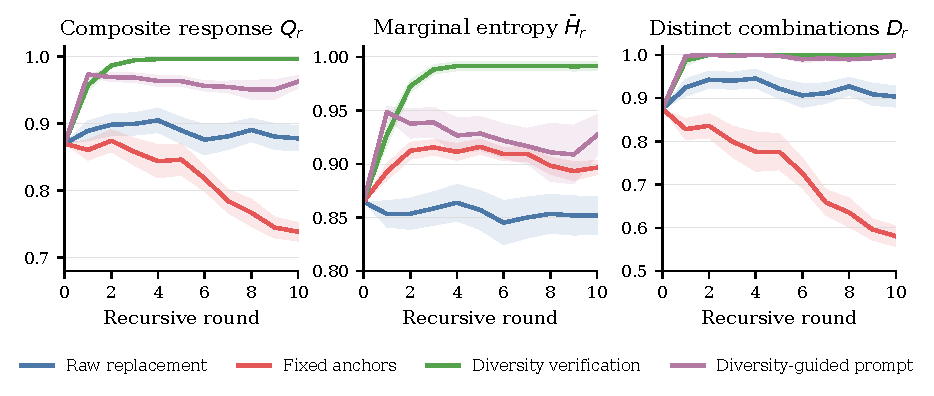
\includegraphics[width=0.97\linewidth]{fig1_recursive_population.pdf}
\caption{One recursive channel, four response laws. Mean trajectories over 16 replicates show the composite score $Q_r$ (left) and its marginal-entropy and distinct-combination components. Verification creates a fast, high plateau; guidance creates an immediate but less uniform plateau; raw replacement drifts; fixed reuse of a small anchor subset preserves marginals while combinations disappear. Shading is $\pm1$ standard error.}
\label{fig:curves}
\end{figure}

\section{Four regimes from one generator}

\begin{center}
\small
\begin{tabular}{lrrrr}
\hline
Intervention & $Q_{10}$ & $g$ & $\bar H_{10}$ & $D_{10}$\\
\hline
Raw replacement & 0.8777 & $+0.0078$ & 0.8519 & 0.9035\\
Fixed anchors & 0.7387 & $-0.1312$ & 0.8966 & 0.5807\\
Diversity verification & 0.9957 & $+0.1259$ & 0.9915 & 1.0000\\
Diversity guidance & 0.9622 & $+0.0923$ & 0.9269 & 0.9974\\
\hline
\end{tabular}
\end{center}

By terminal gain, the arms order as anchors $<$ raw $<$ guidance $<$ verification, sampling the collapse-to-improvement axis. They are not a calibrated one-parameter sweep: each changes a different part of $P_\xi$. Thus they locate regimes in the larger response space, while a future continuous $\rho$ experiment would vary one selector or mixture strength and estimate $\tau_r(\rho)$ directly.

\textbf{Raw replacement is mixed, not steadily collapsing.} Mean response rises to $Q_4=0.9046$ and then gives much back; ten runs end above baseline and six below. Marginal entropy falls while distinct combinations rise. The small endpoint conceals component cancellation and pathwise reversal: a noisy near-neutral regime.

\textbf{Fixed anchoring produces delayed combinatorial collapse.} The mean falls after round five and all terminal gains are negative. Yet entropy \emph{rises} from 0.8648 to 0.8966 while $D_r$ falls from 0.8750 to 0.5807. Reuse keeps values visible but privileges the anchor correlations. This does not indict retaining real data generally; it shows that a narrow fixed archive can preserve parts while concentrating wholes.

\textbf{Verification and guidance improve by different shapes.} Diversity verification reaches $Q_3=0.9941$ and then sits near the finite ceiling; every replicate improves. It creates the closest thing here to an impulsive takeoff. Guidance jumps to $Q_1=0.9729$, then relaxes to a slightly lower and noisier plateau. Both succeed, but selection after generation is more consistent than requesting diversity from generation alone.

These distinctions are visible in the gain--variation plane of Fig.~\ref{fig:geometry}. Verified replicates lie close to the monotone improvement wall. Anchored runs occupy the collapse side but often well above the wall because early gains are later erased. Guided runs improve with more internal motion, and raw replacement clusters near zero terminal gain despite substantial total response. Dividing by $|g|$ would make those near-neutral raw kernels numerically explosive; the unnormalized pair $(g,A)$ remains well behaved.

\begin{figure}[t]
\centering
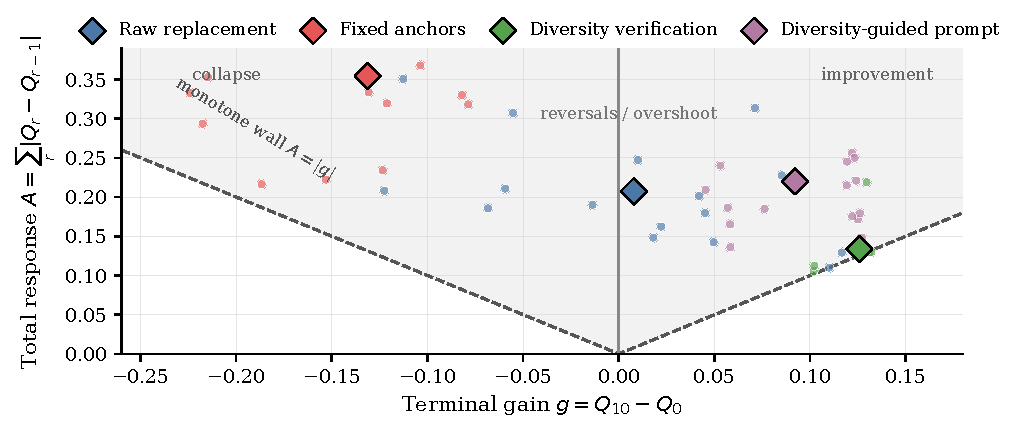
\includegraphics[width=0.90\linewidth]{fig2_response_geometry.pdf}
\caption{Finite-response geometry. Circles are replicates and diamonds are means. Below $A=|g|$ is impossible; height above the monotone wall is response canceled by reversals.}
\label{fig:geometry}
\end{figure}

\section{What this adds to the takeoff picture}

The earlier takeoff note separated terminal gain $g_\xi$ from its kernel $\kappa_\xi$ for each intervention $\xi$ \cite{landersTakeoff}. The modal note tests whether such kernels have exponential sources, although their definition requires none \cite{landersModal}. In the physics analogy a kernel mediates a source \cite{landersEntropy}; here the model is the channel and selection shapes the response, sharpening or spreading it.

\section{Limits and conclusion}

One model, prompt family, ten rounds, and a diversity score cannot establish a capability law; occupancy is only a joint-structure proxy. The experiment instead isolates one principle: recursion has no intrinsic direction. Raw replacement churns, a small archive protects marginals yet destroys combinations, and verification improves rapidly. The empirical object is a family of signed kernels spanning collapse, mixed interiors, and takeoff.

\begin{thebibliography}{9}\scriptsize
\setlength{\parskip}{0pt}

\bibitem{shumailov2024}
I.~Shumailov, Z.~Shumaylov, Y.~Zhao, et al.
\newblock \href{https://doi.org/10.1038/s41586-024-07566-y}{AI models collapse when trained on recursively generated data}.
\newblock \emph{Nature} 631, 755--759, 2024.

\bibitem{alemohammad2024}
S.~Alemohammad, J.~Casco-Rodriguez, L.~Luzi, et al.
\newblock \href{https://openreview.net/forum?id=ShjMHfmPs0}{Self-consuming generative models go MAD}. \emph{ICLR}, 2024.

\bibitem{kazdan2025}
J.~Kazdan, R.~Schaeffer, A.~Dey, et al.
\newblock Collapse or thrive: Perils and promises of synthetic data in a self-generating world.
\newblock \emph{ICML}, PMLR 267:29469--29494, 2025.

\bibitem{landersTakeoff}
J.~R. Landers.
\newblock Takeoff kernels for recursive self-improvement.
\newblock Manuscript, 2026.

\bibitem{landersModal}
J.~R. Landers.
\newblock Beyond single-exponential self-improvement.
\newblock Working draft, 2026.

\bibitem{landersEntropy}
J.~R. Landers.
\newblock The entropy of finite response.
\newblock Manuscript, 2026.

\end{thebibliography}

\end{document}
